\chapter{Abbildungen, Tabellen und Code}
\label{chp:Abbildungen_Tabellen_und_Code}

\section{Grafiken}
\label{sec:Grafiken}

\begin{figure}[ht!]
	\centering
	
\includegraphics[width=0.25\linewidth]{images/example-image.png}
	\caption{Ein importiertes Bild}
	\label{fig:imported}
	Quelle: \citeA{mustermann12}
\end{figure}

\begin{figure}[ht!]
	\centering
	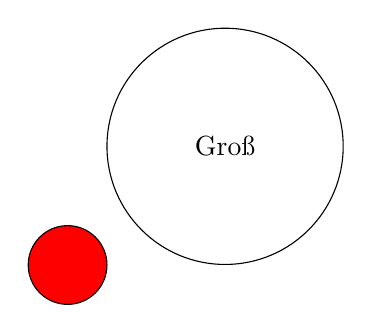
\begin{tikzpicture}
		\node[draw, circle, minimum width=1cm, fill=red] (circle) at (0, 0) {};
		\node[draw, circle, minimum width=3cm, anchor=south] at (2, 0) {Groß};
	\end{tikzpicture}
	\caption{Mit TikZ gezeichnete Kreise}
	\label{fig:drawn}
\end{figure}

\section{Tabellen}
\label{sec:Tabellen}

\begin{table}[ht!]
	\centering
	\begin{tabular}{l|ccc}
		Test & Feld & Feld & Feld \\
		\hline
		Eins & 1 & 2 & 3 \\
		Zwei & 4 & 5 & 6 \\
		Drei & 7 & 8 & 9 \\
	\end{tabular}
	\caption{Einfache Beispieltabelle}
	\label{tab:plaintable}
\end{table}

\begin{table}[ht!]
	\centering
	\rowcolors{2}{gray!25}{white}
	\begin{tabular}{ccc}
		\toprule
		\belowrulesepcolor{gray!50}
			\rowcolor{gray!50}
		& \bfseries Head & \bfseries Head \\
		\aboverulesepcolor{gray!50}
		\midrule
		x & Wert & Wert \\
		x & Wert & Wert \\
		x & Wert & Wert \\
		x & Wert & Wert \\
		\aboverulesepcolor{gray!25}
		\bottomrule
	\end{tabular}
	\caption[Fancy Tabelle]{Längerer Tabellentitel, der nicht im Verzeichnis steht}
	\label{tab:fancytable}
\end{table}

\section{Quelltext}
\label{sec:Quelltext}

Einem Listing den Parameter \emph{float} zu geben verhindert, dass er über Seiten hinweg gebrochen wird.
Dies kann bei kürzerem Code nützlich sein, um die visuelle Struktur beizubehalten.

\begin{lstlisting}[
	caption={Code in Standardsprache aus style.tex (z.\,B. Python)},
	label={lst:default},
	float={ht!}
]
	# Standard Code, hier: Python
	print("Hello World!")
\end{lstlisting}

\begin{lstlisting}[
	language=Java,
	caption={Code in Java},
	label={lst:java},
	float={ht!}
]
	// Java
	System.out.println("Hello World!");
\end{lstlisting}

\begin{lstlisting}[
	language=None,
	caption={Code ohne Highlighting},
	label={lst:nohighlighting},
	float={ht!}
]
	# Kein Highlighting
	print("Hello World!")
\end{lstlisting}
